\documentclass[10pt,a4paper]{article}
\usepackage[margin=2.2cm]{geometry}
\usepackage[T1]{fontenc}
\usepackage{lmodern}
\usepackage{graphicx}
\usepackage{booktabs}
\usepackage{longtable}
\usepackage{xcolor}
\usepackage{caption}
\usepackage{float}
\usepackage[hidelinks]{hyperref}
\definecolor{ok}{HTML}{008300}
\definecolor{part}{HTML}{B07800}
\definecolor{no}{HTML}{E34948}
\graphicspath{{../figures/}}
\captionsetup{font=small,labelfont=bf}
\setlength{\parskip}{0.35em}
\newcommand{\TpchSpread}{3.6}
\newcommand{\TpcdsSpread}{5.0}
\newcommand{\TpchScans}{3.8}
\newcommand{\TpchJoins}{3.5}
\newcommand{\TpcdsScans}{7.4}
\newcommand{\TpcdsJoins}{6.8}
\newcommand{\QueriesProv}{433,107,731}
\newcommand{\QueriesServ}{8,244,381}
\newcommand{\CachedRestoredProv}{96.2}
\newcommand{\IdealHitProv}{63.1}
\newcommand{\IdealHitServ}{38.6}
\newcommand{\RealHitProv}{33.6}
\newcommand{\RealHitServ}{14.8}
\newcommand{\IdealSavedProv}{25.1}
\newcommand{\IdealSavedServ}{17.6}
\newcommand{\RealSavedProv}{8.3}
\newcommand{\RealSavedServ}{1.2}
\newcommand{\ModelExplainsProv}{97.5}
\newcommand{\ModelExplainsServ}{99.1}
\newcommand{\AllTableSetsMean}{97,637}
\newcommand{\TtlTenMinHitProv}{56.3}
\newcommand{\TtlTenMinSavedProv}{14.9}
\newcommand{\TtlOneHourHitProv}{59.8}
\newcommand{\TtlOneHourSavedProv}{19.8}
\newcommand{\TtlTenMinHitServ}{27.0}
\newcommand{\TtlTenMinSavedServ}{11.9}
\newcommand{\TtlOneHourHitServ}{32.9}
\newcommand{\TtlOneHourSavedServ}{16.1}


\title{\textbf{Is TPC Still Not Enough?}\\[0.3em]
\large Replicating the Amazon Redshift fleet study (VLDB 2024) on the public Redset trace,\\
and measuring what an ideal result cache would save}
\author{Mohamed Abderrahmane Heouaine}
\date{October 2026}

\begin{document}
\maketitle

\begin{abstract}
\noindent
van Renen et al.\ (PVLDB 17(11), 2024) argue, from internal Amazon Redshift telemetry, that the TPC-H and TPC-DS benchmarks no longer match what cloud data warehouses run: write-heavy pipelines, repetitive queries, bursty load and long-tailed distributions. With the paper, Amazon released \emph{Redset}, a trace of queries from 200 provisioned and 200 serverless clusters over three months of 2024. This report asks whether the paper's conclusions hold on that public data. I rebuilt the paper's metrics as tested SQL over the full trace (\QueriesProv{} provisioned and \QueriesServ{} serverless queries) on a single laptop with DuckDB, and compared 29 quantitative claims: 17 are confirmed, 7 partially confirmed, 5 not confirmed. The core argument survives: about two thirds of the runtime goes to writes, the runtime tail is even longer than reported, and in the median provisioned cluster 79\,\% of queries repeat (paper: 80\,\%). The query mix (fewer selects), the usage of CTAS tables and the number of distinct table sets differ markedly. Three properties of the trace had to be handled first; the most consequential is that result-cache hits are logged as \texttt{other}, which hides them from every select-based metric. As an extension, I replay every select against an ideal result cache with table-level invalidation: it would answer \IdealHitProv\,\% of provisioned selects instead of the \RealHitProv\,\% Redshift answered, and save \IdealSavedProv\,\% of select runtime instead of \RealSavedProv\,\%. The model classifies \ModelExplainsProv\,\% of the real cache hits as hits, which validates it.
\end{abstract}

\section{Introduction}

Benchmarks shape what database systems optimize. The paper replicated here \cite{tpc} compares one month of telemetry from the provisioned Amazon Redshift fleet with TPC-H and TPC-DS and concludes that a modern benchmark must model writes, repetition, elasticity and long tails. Its numbers cannot be checked directly: the telemetry is private. The authors released a public dataset, Redset \cite{redset}, ``as a basis for building more realistic benchmarks''. It is a different sample (other clusters, a later period, serverless included) with fewer columns (no query text, no filters, no memory, no table statistics).

This is therefore a \emph{conceptual replication}: the same metrics, recomputed independently on different data from the same system. For each quantitative claim the question is whether it survives on the data anyone can download. The contributions are:
\begin{enumerate}\setlength{\itemsep}{0pt}
\item an open pipeline (DuckDB SQL, about one hour on a 16-thread laptop) that recomputes the paper's Sections 3--5 on the full Redset, with unit tests on hand-made traces;
\item a scorecard of 29 claims for the provisioned and serverless variants (Table~\ref{tab:claims});
\item three properties of Redset that change the results if ignored (Section~\ref{sec:traps});
\item an extension that the paper motivates but does not quantify: the hit rate and saved runtime of an ideal result cache, validated against Redshift's real cache, and its sensitivity to an eviction timeout (Section~\ref{sec:cache}).
\end{enumerate}

\section{Data and method}

\paragraph{Redset.} One row per query: cluster, user and database ids, arrival time, compile, queue and execution times, query type, a hash of the query's features (\texttt{feature\_fingerprint}), abort and result-cache flags, numbers and ids of the tables read and written, megabytes scanned and spilled, and the numbers of joins, scans and aggregations in the plan. Clusters were sampled to cover all levels of activity, so fleet-wide shares are shares \emph{of this sample}. After restricting to 1 March--30 May 2024 (the trace ends at midnight on 31 May; 81 rows fall outside), it holds 441.4 million queries.

\paragraph{Pipeline.} The 17.7\,GB of Parquet files are loaded once into a typed DuckDB table (fingerprints hashed to 64-bit integers, table-id strings parsed into lists). Each metric is a SQL query whose result is saved as a CSV; every number below is read from those files by a script, not typed by hand. TPC-H and TPC-DS run in DuckDB at scale factor 10 on the same laptop; absolute runtimes are therefore not comparable with the paper's 10-node cluster at SF\,3000, only the shape of their distribution and the plan operators per query.

\paragraph{Metric definitions.} Runtime is the execution time. \emph{Spikiness} is described in the paper as ``the sum of the root mean square errors between the current and previous day'' without a normalization. I normalize each series to sum to one and sum the absolute differences of consecutive values (the RMSE of two scalars), over the days of a month (daily) or the 24 hours of the day (hourly). On the aggregated provisioned fleet this gives 0.11 daily and 0.11 hourly against the paper's 0.12 and 0.09, which supports this reading. \emph{Repetition} follows the paper: (queries $-$ distinct queries) / queries in a window, with the fingerprint standing in for the query. Redset's documentation warns that the fingerprint overestimates repetition, so it sits between the paper's ``query'' and ``query template'' metrics.

\subsection{Three properties of the trace}\label{sec:traps}
\begin{enumerate}\setlength{\itemsep}{0pt}
\item \textbf{Result-cache hits are logged as \texttt{other}}, with no fingerprint and no tables, plus a pointer to the query that produced the result (a select in 99.8\,\% of cases). Left as is, the real cache hit rate among selects is 0\,\%, selects are undercounted by a third and repetition is underestimated. I restore them as selects with their source's fingerprint and tables (\CachedRestoredProv\,\% of provisioned hits have their source in the trace).
\item \textbf{The trace ends on 30 May.} Keeping 31 May adds an almost empty day and a fake drop in load.
\item \textbf{Every CTAS creates a new table id} (25.36 M creations, 25.34 M distinct target ids). Re-creation of ``the same table'' is measured through the CTAS statement's fingerprint instead. The same effect on staging tables inflates the number of distinct table sets (Section~\ref{sec:tables}).
\end{enumerate}

\section{Results}

Table~\ref{tab:claims} lists every claim. The sections below discuss them in the paper's order.

{\small
\setlength{\tabcolsep}{4pt}
\begin{longtable}{@{}l p{6.6cm} r r r l@{}}
\caption{Replication scorecard. Paper values are from the paper's tables and text; Redset values are computed on the full trace. ``Partial'': same direction, clearly different size or a proxy metric.}\label{tab:claims}\\
\toprule
\S & Claim & Paper & Provisioned & Serverless & Verdict \\
\midrule
\endfirsthead
\toprule
\S & Claim & Paper & Provisioned & Serverless & Verdict \\
\midrule
\endhead
\csname @@input\endcsname claims.tex
\bottomrule
\end{longtable}
}

\subsection{Queries: writes dominate, and the tail is longer}
\begin{figure}[H]
\centering
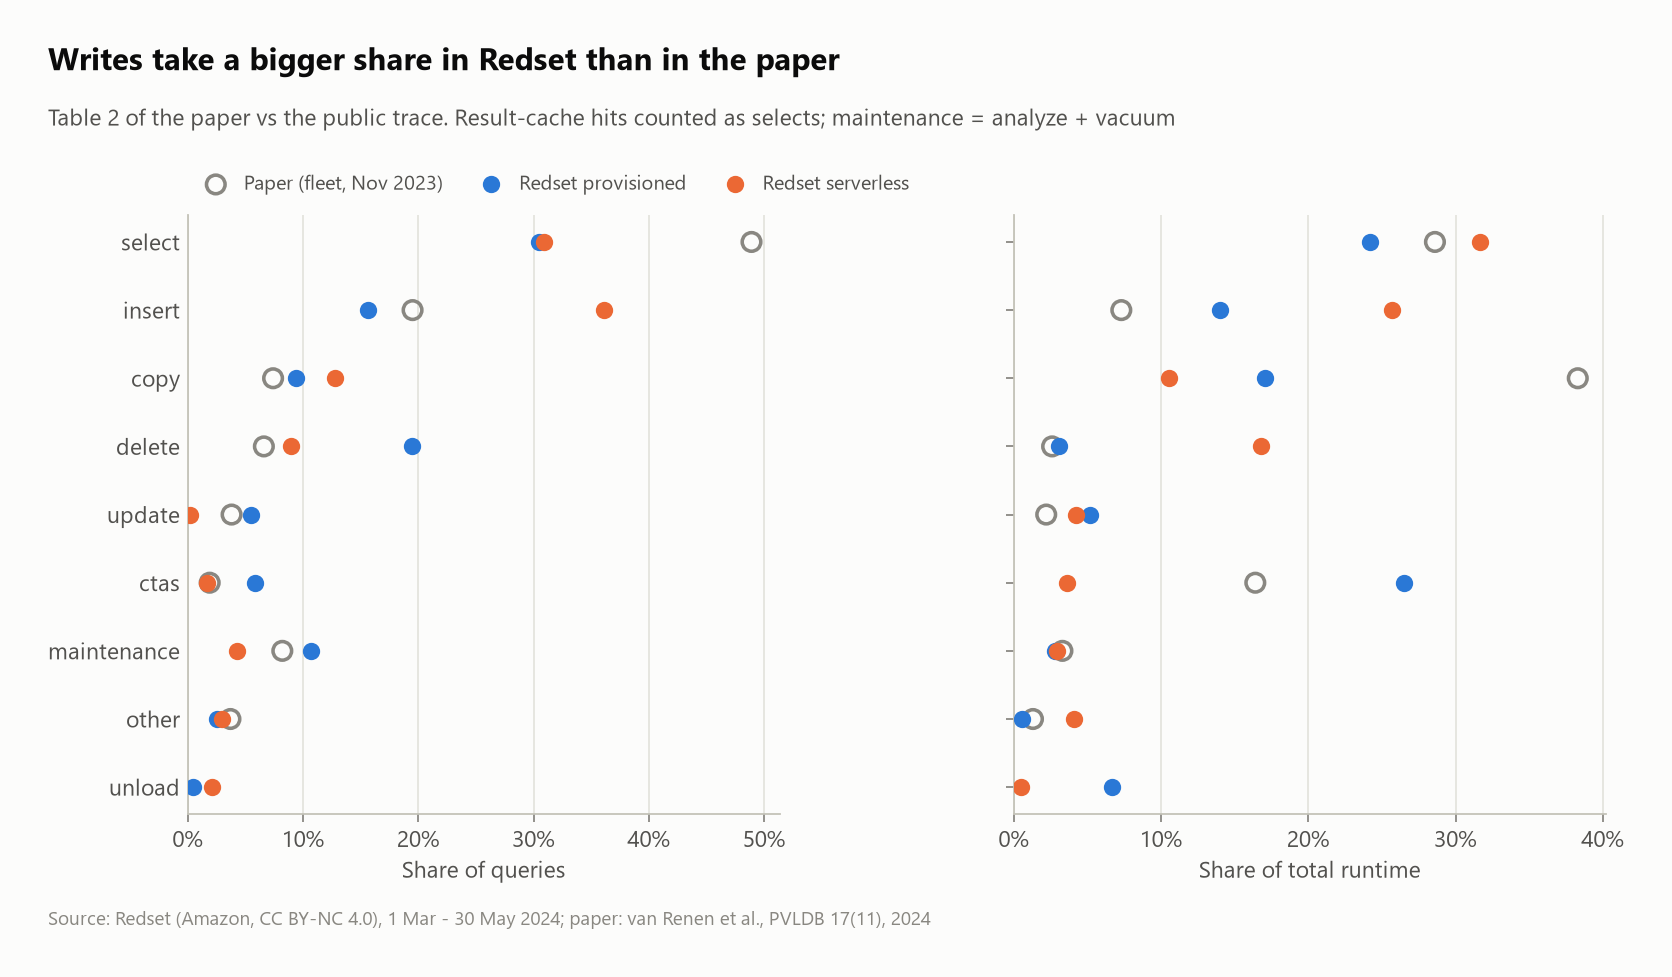
\includegraphics[width=0.92\linewidth]{query_types.png}
\caption{Share of queries and of runtime per query type (the paper's Table 2).}\label{fig:types}
\end{figure}

The paper's ``analytics = updates'' holds strongly (Figure~\ref{fig:types}). Writes take 65.8\,\% of provisioned runtime (paper: 66.8\,\%). Only 30.5\,\% of queries are selects, against 48.9\,\% in the paper, so on the public trace writes dominate the query count even more. CTAS statements take 26.5\,\% of provisioned runtime (paper: 16.4\,\%) but only 3.6\,\% on serverless, where plain inserts dominate.

Runtimes are short and heavy-tailed (Figure~\ref{fig:buckets}). 62.4\,\% of provisioned queries finish within 100\,ms (paper: 62.0\,\%), while 0.005\,\% of queries run longer than an hour and take 12.7\,\% of the runtime. The paper's Table~3 gives 15.9\,\% for that bucket; its text says ``$\approx$25\,\%''. The ratio of the 99.9th percentile to the median is 7{,}483 (provisioned) and 7{,}066 (serverless), against 2{,}030 in the paper. TPC is narrow by comparison: the 90th percentile of the 22 TPC-H runtimes is \TpchSpread$\times$ their median (TPC-DS: \TpcdsSpread$\times$), against 38$\times$ on Redset provisioned. Queries are also simpler than TPC's. An executed Redset query has 1.31 scans and 0.52 joins on average (paper: 2.03 and 0.53), while a TPC-H query in DuckDB has \TpchScans{} scans and \TpchJoins{} joins (TPC-DS: \TpcdsScans{} and \TpcdsJoins).

\begin{figure}[H]
\centering
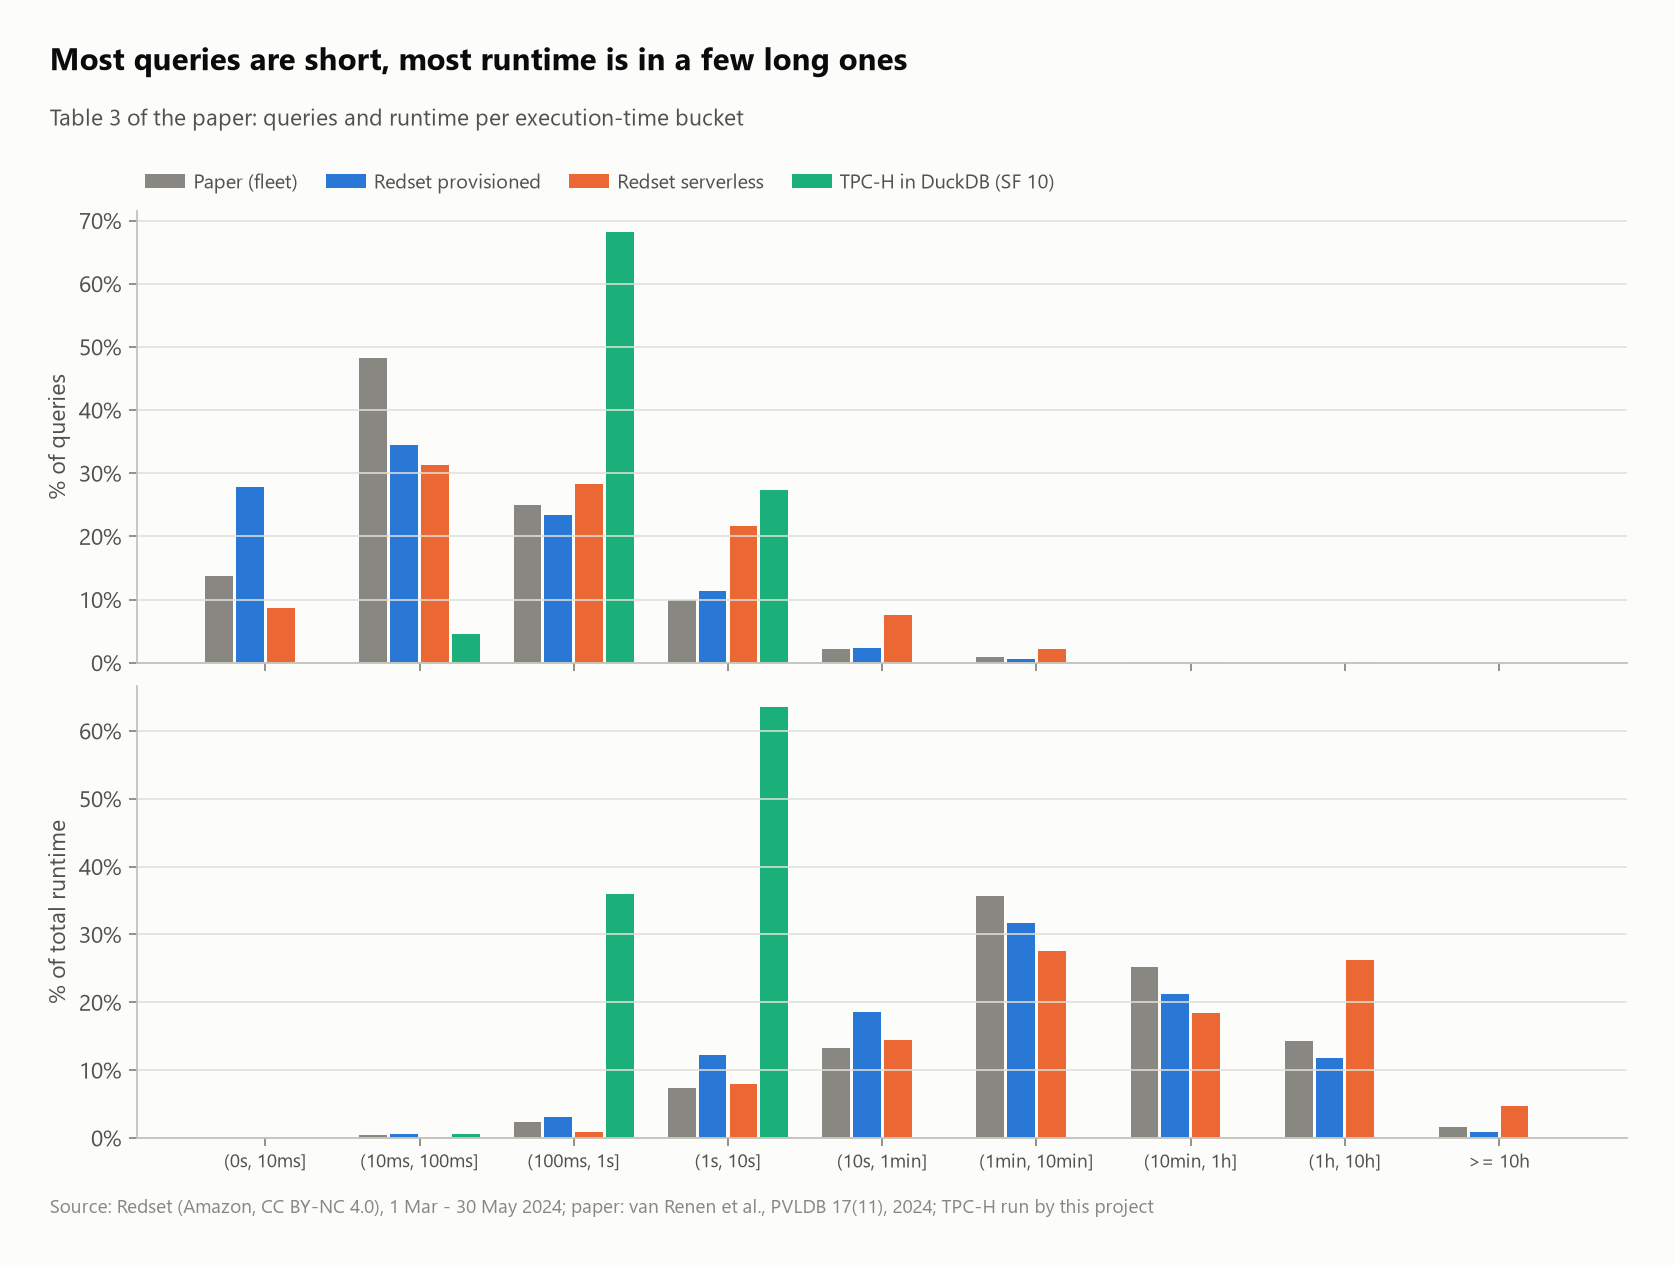
\includegraphics[width=0.92\linewidth]{runtime_buckets.png}
\caption{Queries and runtime per execution-time bucket (the paper's Table 3), with TPC-H run in DuckDB.}\label{fig:buckets}
\end{figure}

\subsection{Workloads: a stable fleet of unstable clusters}
\begin{figure}[H]
\centering
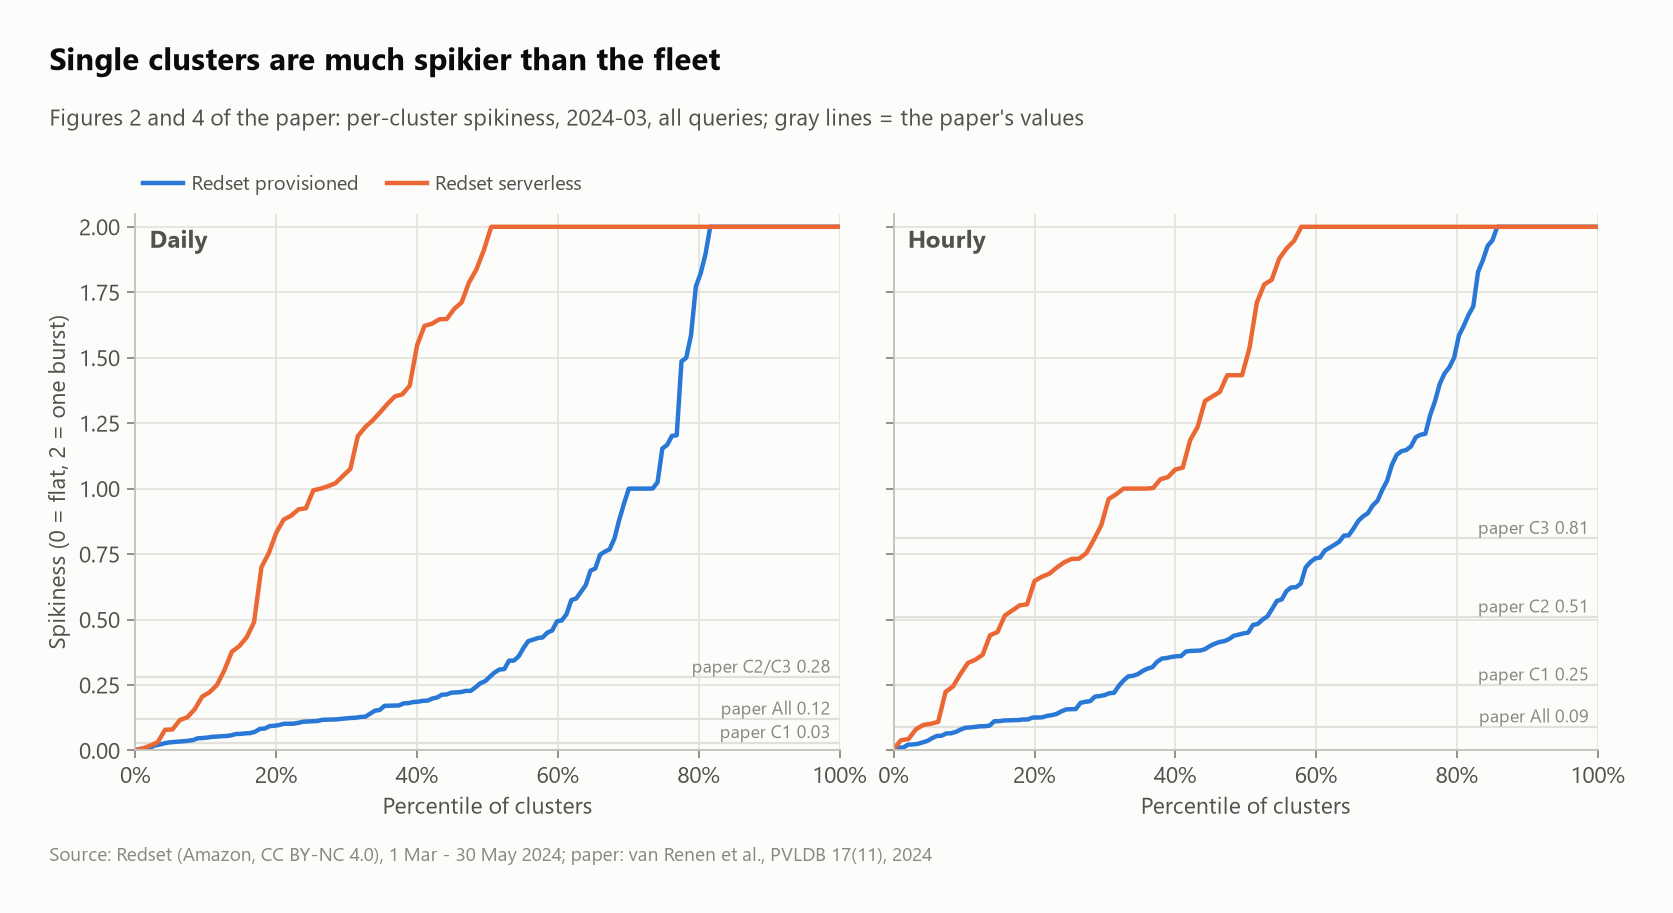
\includegraphics[width=0.92\linewidth]{spikiness.png}
\caption{Spikiness per cluster in March 2024 (the paper's Figures 2 and 4).}\label{fig:spiky}
\end{figure}

Aggregated over all clusters, the load is as stable as in the paper (daily spikiness 0.11 vs 0.12). Single clusters are spikier (Figure~\ref{fig:spiky}). Half of the provisioned clusters are at most as spiky as the paper's ``typical'' cluster C2, where the paper reports 75\,\%. Serverless clusters are far burstier (median daily spikiness 1.96 out of 2): many run a few jobs a day. This is what serverless is for, and it is a workload no TPC run reproduces. Fleet-level stability also varies by month: serverless daily spikiness is 0.15 in March but 0.69 in April.

\subsection{Repetition: confirmed, with nuances on timing}
\begin{figure}[H]
\centering
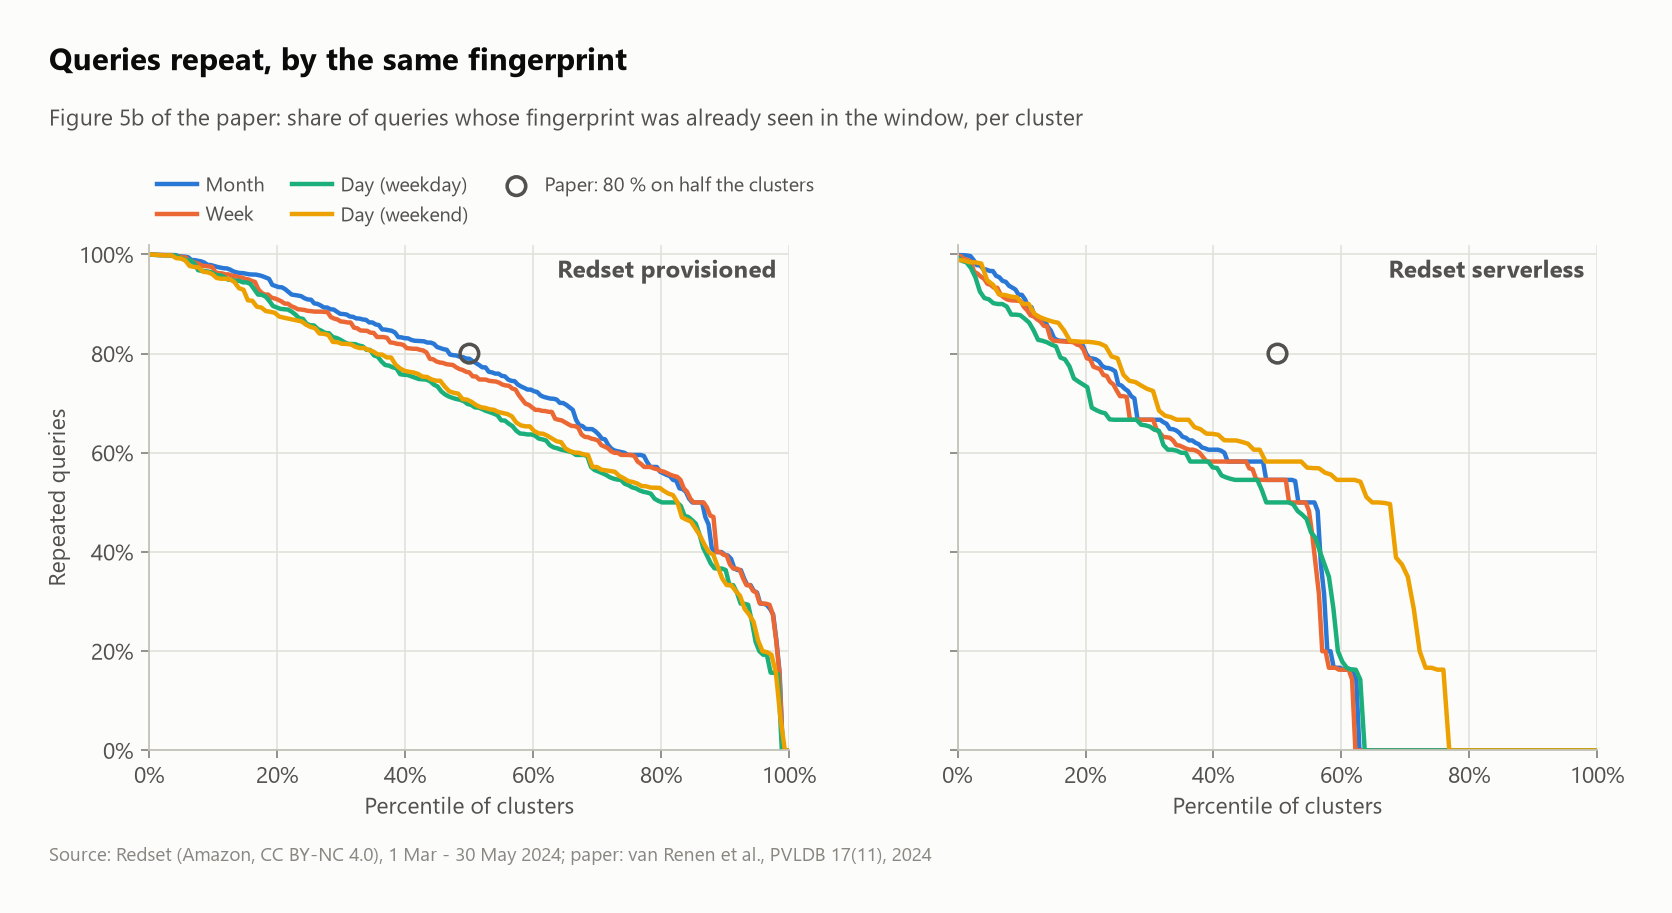
\includegraphics[width=0.92\linewidth]{repetition.png}
\caption{Share of repeated queries per cluster, for several windows (the paper's Figure 5b).}\label{fig:rep}
\end{figure}

In the median provisioned cluster, 79\,\% of a month's queries repeat an earlier fingerprint (paper: 80\,\%; Figure~\ref{fig:rep}). The serverless median is lower (54.5\,\%), and 37.5\,\% of serverless clusters show no repetition at all in the month. As in the paper, long queries repeat: in the median cluster, 82\,\% of the queries whose fingerprint runs 10\,min--10\,h are repeats, against 32\,\% under 10\,ms. The timing claim depends on how one reads it. Per cluster, the median gap between repeats of a select is 42\,s (paper: under 100\,s). Per repeating query, the median gap is about ten minutes. The longest per-cluster median is 1.0 day, not 12.

\subsection{Tables and CTAS: the clearest disagreements}\label{sec:tables}
70.8\,\% of CTAS statements run once in a given week (paper: 66\,\%), but their tables are not single-use: only 8.1\,\% are read by exactly one query (paper: 80\,\%). 58.9\,\% are read by 2--5 queries and 24.7\,\% by none, and 17.6\,\% of all queries read a CTAS-created table (paper: 40\,\%). The paper reports 23.5 distinct table sets in busy clusters. Over 10 randomly sampled busy cluster-months, Redset gives a median of 1{,}438 even after dropping tables read on a single day, and a mean of \AllTableSetsMean{} with all tables. Both differences may come from how tables are identified: the paper probably sees stable table names, while Redset ids change with every re-creation. Same-day writes agree: 76.9\,\% of tables that receive inserts on a day receive no delete that day (paper: 80\,\%).

\section{Extension: what would an ideal result cache save?}\label{sec:cache}
The paper reports a cache hit rate of $\approx$20\,\%, that $\approx$80\,\% of queries repeat, and a breakdown of why repeats miss. Redset allows the counterfactual. I replay every select of every cluster in arrival order. A select is an \emph{ideal hit} if
(1) the same fingerprint ran before on the cluster,
(2) it reads no system or external table,
(3) the previous run had finished when it arrives, and
(4) no write to any table it reads committed since the previous run \emph{started}. A write committing during the previous run makes that result stale under snapshot isolation.
The last relevant commit is found with a single ASOF join of the per-table read list against the write log, which avoids a quadratic scan. A real hit reports $\sim$0\,ms, so saved runtime uses the median runtime of the fingerprint's real executions. The rules are unit-tested on hand-made traces, including the paper's 3/8 repetition example.

\begin{figure}[H]
\centering
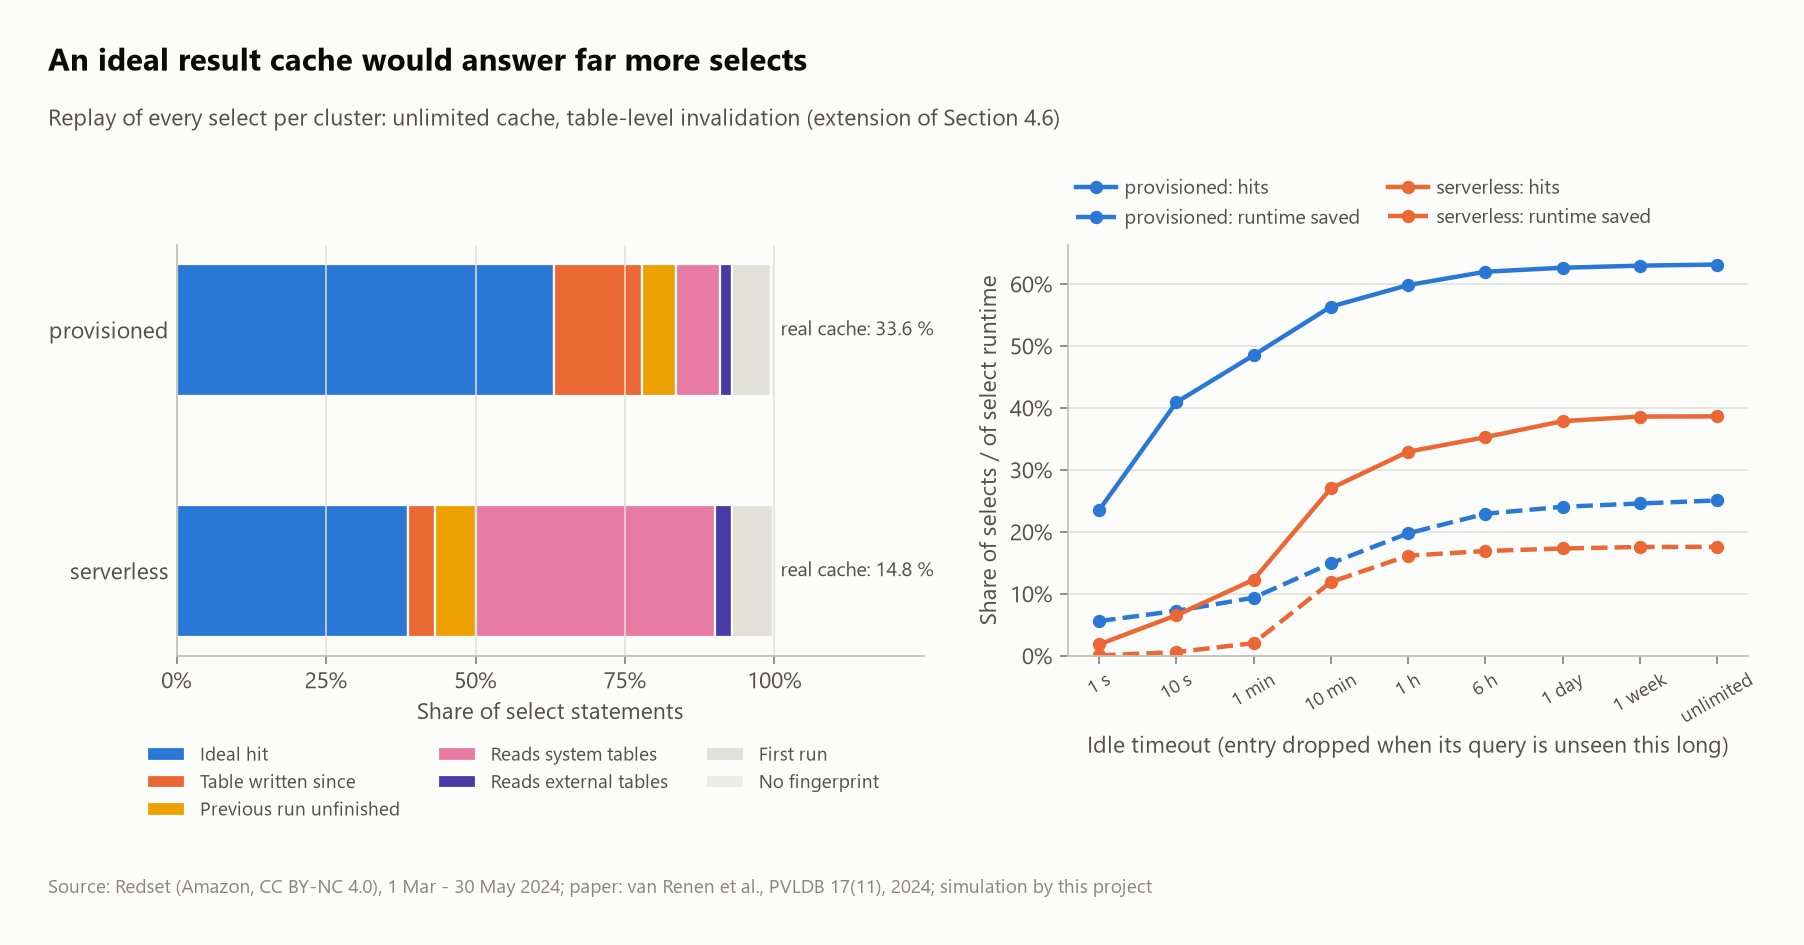
\includegraphics[width=0.98\linewidth]{cache.png}
\caption{Left: every select classified by the ideal cache. Right: hits and saved runtime under an idle timeout.}\label{fig:cache}
\end{figure}

\paragraph{Validation.} Of the selects Redshift really answered from its cache, the model classifies \ModelExplainsProv\,\% (provisioned) and \ModelExplainsServ\,\% (serverless) as ideal hits. The model is therefore not missing a way the real cache works.

\paragraph{Results.} An ideal cache would answer \IdealHitProv\,\% of provisioned selects, against the \RealHitProv\,\% really answered. It would save \IdealSavedProv\,\% of select runtime instead of \RealSavedProv\,\%, three times more (Figure~\ref{fig:cache}). On serverless, the figures are \IdealHitServ\,\% vs \RealHitServ\,\% of selects and \IdealSavedServ\,\% vs \RealSavedServ\,\% of runtime. Real misses among repeating selects (63.9\,\%, paper: $\approx$60\,\%) break down as follows. Writes since the previous run explain 24.8\,\% of them (paper: 54\,\%), system tables 12.4\,\% (paper: 14\,\%) and external tables 3.3\,\% (paper: 4\,\%). The remaining ideal hits that Redshift missed are 30.4\,\% of provisioned selects and 16.9\,\% of select runtime. They cover causes Redset does not expose: non-deterministic functions, oversized results, eviction and cache scope.

\paragraph{Timeouts.} The hits are cheap queries repeated quickly, the savings are expensive queries repeated slowly. An entry dropped after 10 idle minutes keeps \TtlTenMinHitProv\,\% of selects as hits (89\,\% of the ideal) but saves only \TtlTenMinSavedProv\,\% of runtime (about 60\,\% of the ideal); one hour gives \TtlOneHourHitProv\,\% and \TtlOneHourSavedProv\,\%. A cache sized by hit rate would therefore miss most of the runtime it could save; retention should be weighted by the cost of the query.

\section{Threats to validity}
\begin{itemize}\setlength{\itemsep}{0pt}
\item \textbf{Different sample and period.} Redset is a biased sample of clusters, from 2024, while the paper uses November 2023; serverless is a different product. Some disagreements may be real differences between samples rather than errors in either study.
\item \textbf{Proxies.} The fingerprint is not the query text (it overestimates repetition); table ids are not table names; filters, memory, data types, data skew and storage formats (the paper's Section 5) cannot be measured at all.
\item \textbf{Interpretation.} The spikiness normalization and the per-cluster reading of the repeat-gap claim are my choices; both are documented and the first is checked against the paper's fleet value.
\item \textbf{TPC side.} DuckDB on a laptop at SF\,10 is not Redshift at SF\,3000; only distribution shapes and plan operators are compared.
\item \textbf{Cache model.} It ignores result size limits, eviction under memory pressure and non-deterministic functions, so it is an upper bound. The 97\,\% agreement with real hits only shows that it does not \emph{miss} real behavior.
\end{itemize}

\section{Conclusion}
On the public trace, the paper's central message holds. Cloud warehouse workloads are write-heavy, repetitive and long-tailed, and TPC captures none of that: TPC-H's runtime spread is ten times narrower and its queries scan three times more tables. Several specific numbers do not transfer: the query mix, CTAS usage and table sets. A benchmark built from ``the'' fleet numbers would encode one sample, which supports the paper's own call for a configurable benchmark generator. The cache extension turns the paper's qualitative remark into a number: two thirds of the select runtime that an ideal cache could save is not saved today, and recovering it needs cost-aware retention more than a larger hit rate. Everything (SQL, tests, figures and this report) regenerates from the raw trace with one command.

\begin{thebibliography}{9}\small
\bibitem{tpc} A. van Renen, D. Horn, P. Pfeil, K. Vaidya, W. Dong, M. Narayanaswamy, Z. Liu, G. Saxena, A. Kipf, T. Kraska. \emph{Why TPC Is Not Enough: An Analysis of the Amazon Redshift Fleet.} PVLDB 17(11): 3694--3706, 2024. doi:10.14778/3681954.3682031
\bibitem{redset} Amazon. \emph{Redset}, \url{https://github.com/amazon-science/redset}. CC BY-NC 4.0.
\bibitem{duckdb} M. Raasveldt, H. M\"uhleisen. \emph{DuckDB: an Embeddable Analytical Database.} SIGMOD 2019.
\end{thebibliography}
\end{document}
